\section{Application of probabilistic catalogs for population studies}
\lb{sec:dNdS}



\begin{figure*}[h]
%\hspace*{-1cm}
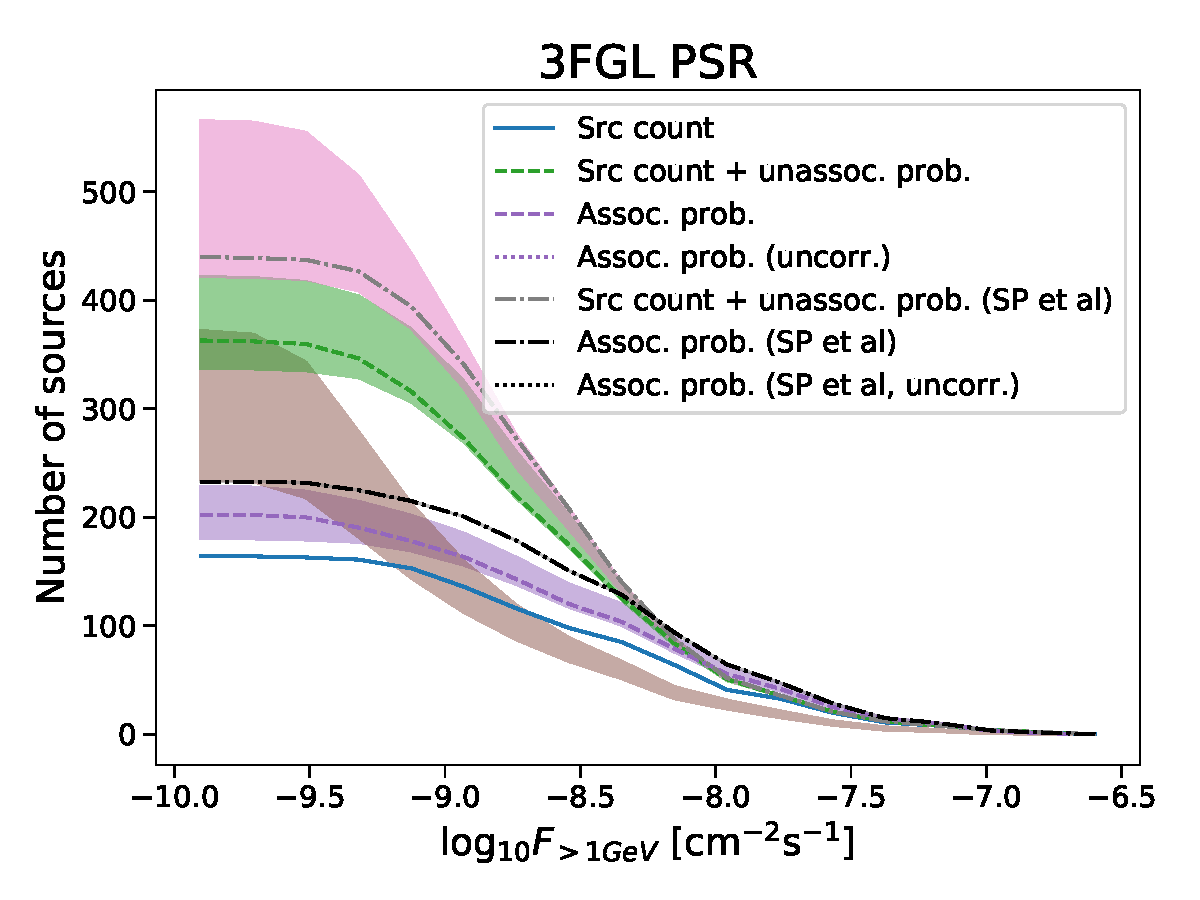
\includegraphics[width=0.4\textwidth]{plots/N_logS_3FGL_PSR_SazP.pdf}
%\hspace*{-1cm}
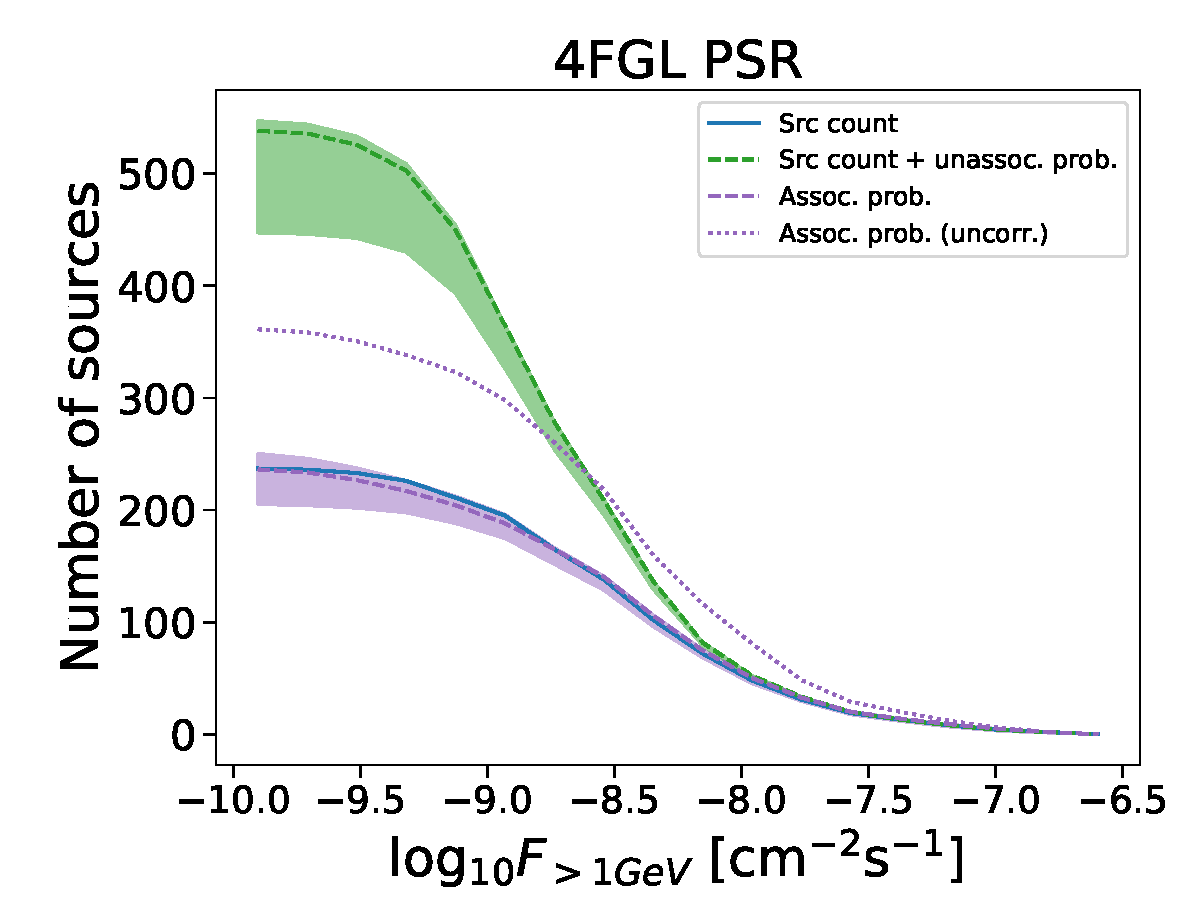
\includegraphics[width=0.4\textwidth]{plots/N_logS_4FGL_PSR.pdf} \\
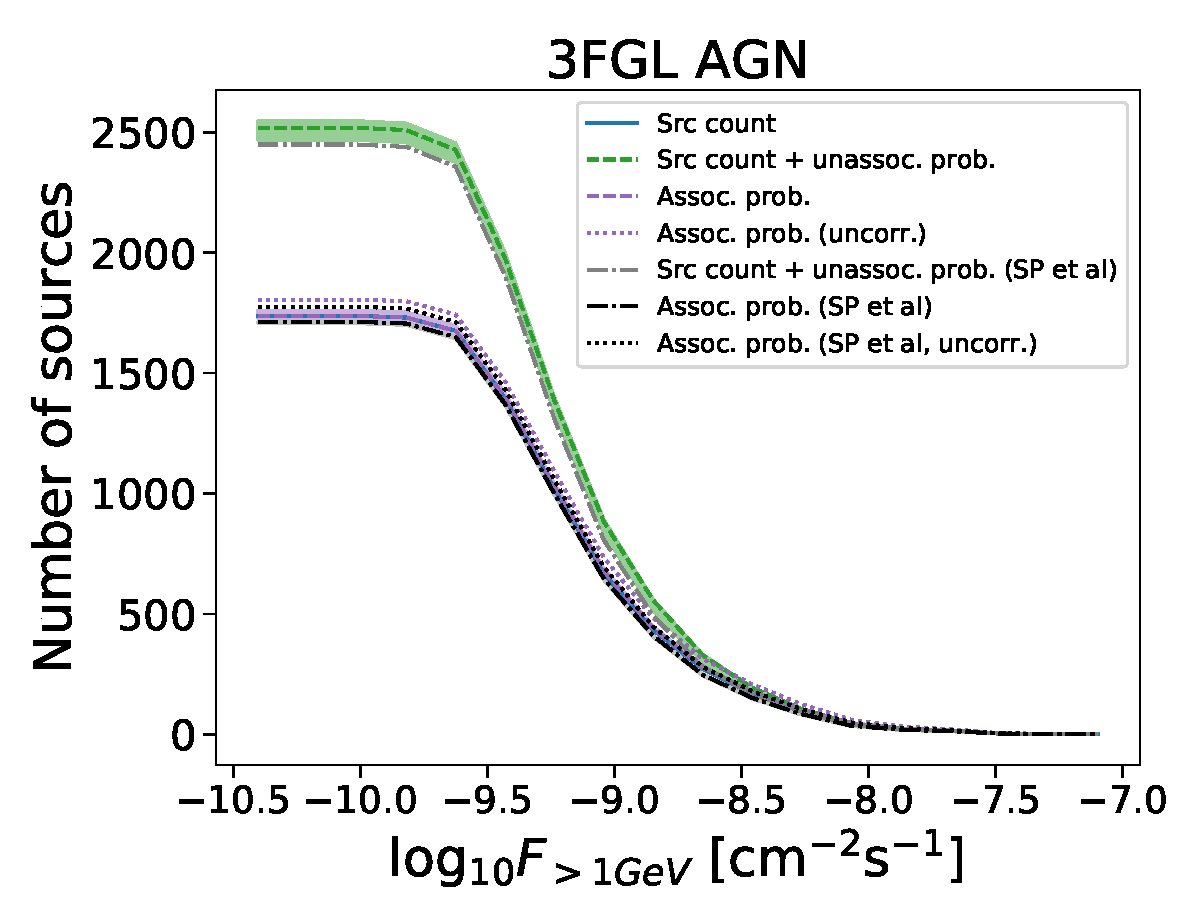
\includegraphics[width=0.4\textwidth]{plots/N_logS_3FGL_AGN_SazP.pdf}
%\hspace*{-1cm}
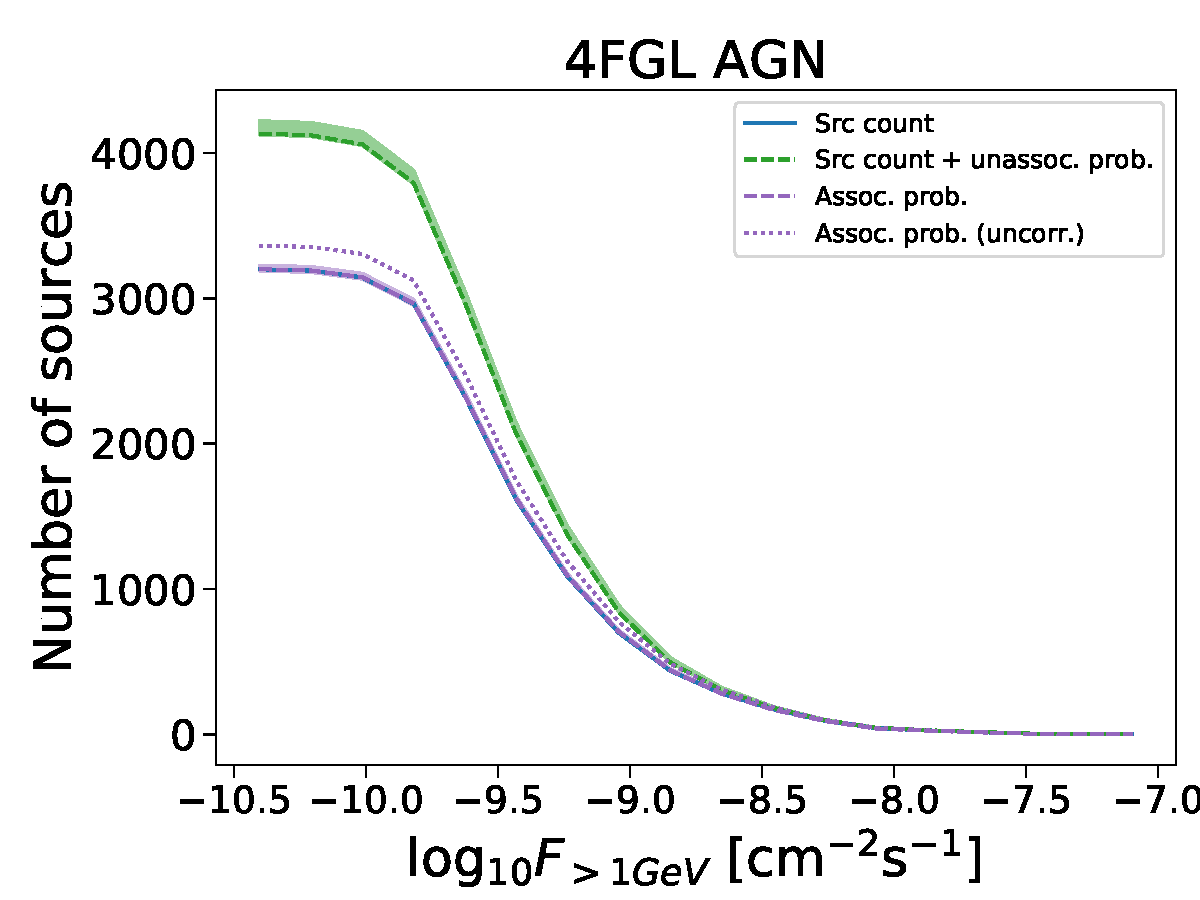
\includegraphics[width=0.4\textwidth]{plots/N_logS_4FGL_AGN.pdf}
\caption{Cumulative number of sources as a function of their flux.}  
\label{fig:logN_logS}
\end{figure*}


\begin{figure}[h]
%\hspace*{-1cm}
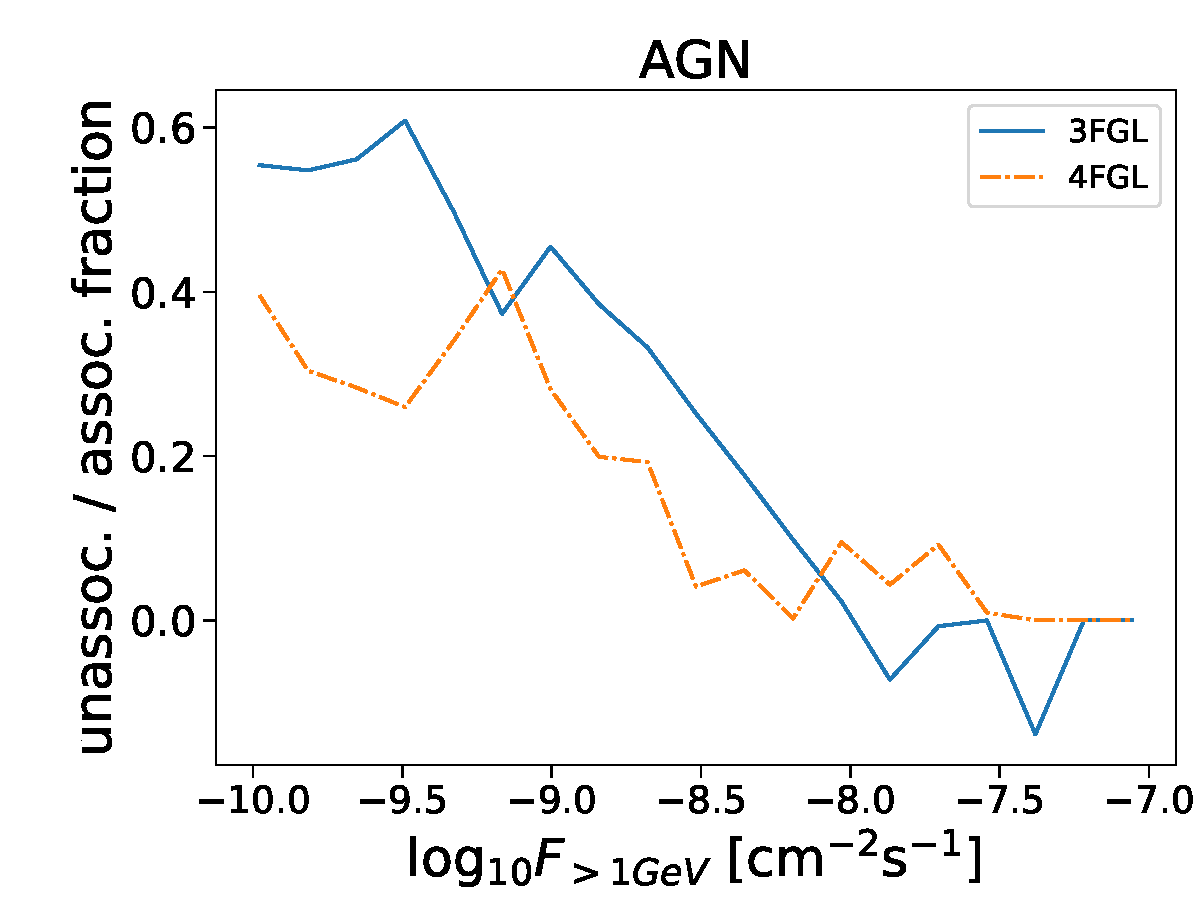
\includegraphics[width=0.4\textwidth]{plots/logN_logS_diff_AGN_unweighted.pdf}
%\hspace*{-1cm}
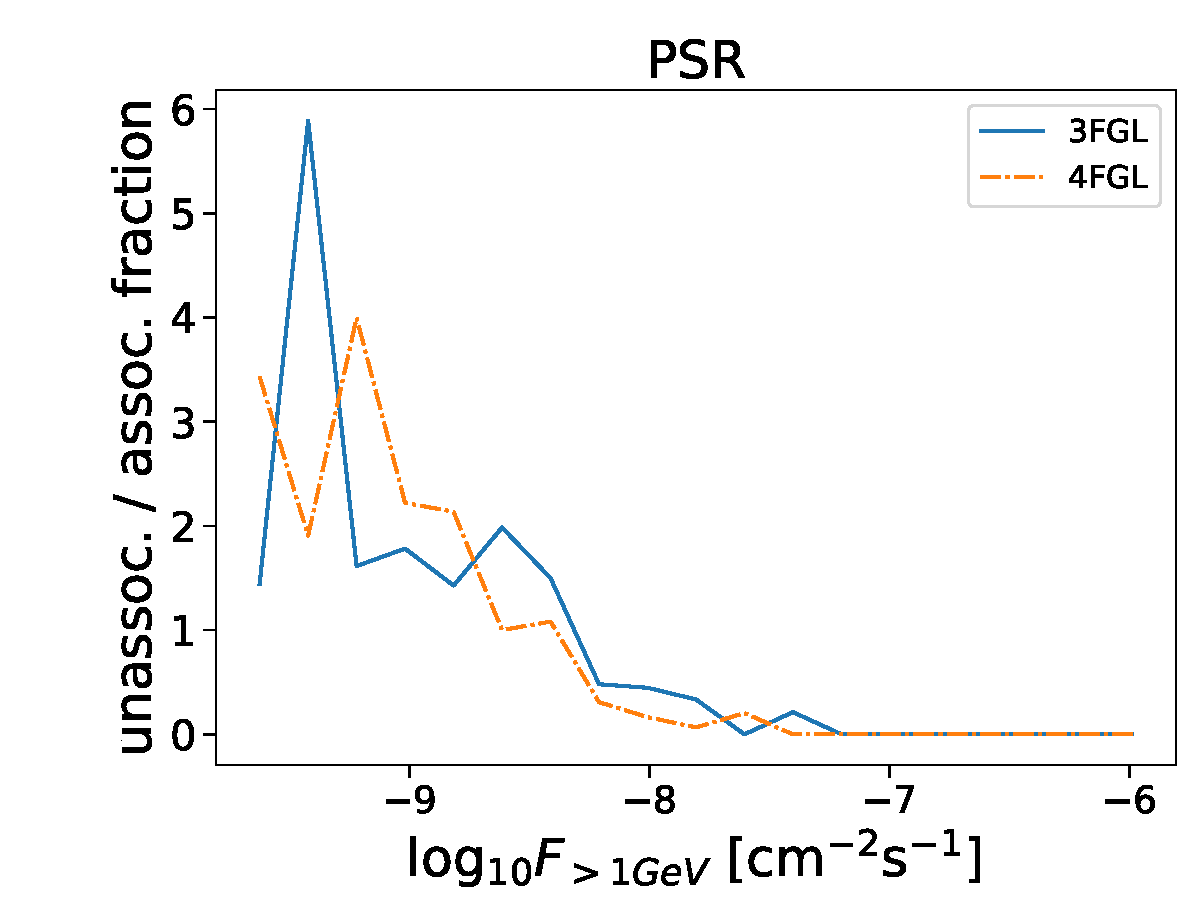
\includegraphics[width=0.4\textwidth]{plots/logN_logS_diff_PSR_unweighted.pdf}
\caption{Fraction of unassociated sources relative to associated ones.}  
\label{fig:unass_vs_ass_frac}
\end{figure}



In this Section we show how probabilistic catalogs can be used, for instance, for population studies.
One of the most important questions in gamma-ray astronomy is contribution of point sources, e.g., AGNs, to the extragalactic gamma-ray
flux:
if most of the extra-galactic emission is explained by the point sources, then one can put stringent constraints, e.g., on 
dark matter annihilation into gamma rays, on evaporation of primordial black holes, and on the origin of astrophysical high energy neutrino flux.
In particular, it is important to understand the contribution to the population of AGNs from the unassociated sources.
A probabilistic catalog provides an answer to the question: how many sources among the unassociated ones are expected to belong to different classes, such as pulsars or AGNs. 
One can calculate the total expected number of AGNs or pulsars among the unassociated sources, or calculate the contribution as a function of one or more parameters.
In this section we determine the numbers of AGNs and pulsars as a function of their flux.

In Figure \ref{fig:logN_logS} we show the cumulative number of AGNs and pulsars with flux above 1 GeV larger than the
value on the x-axis.
We plot the number of associated sources using solid (3FGL) and dash-dotted (4FGL) lines.
We also add unassociated sources weighted by AGN or PSR probabilities in order to estimate the total number of AGNs and pulsars
among the detected sources.
Dashed and dotted lines show the contribution of unassociated sources in 3FGL and 4FGL respectively using LR algorithm.
The bands show the envelop for the predicted number of sources using all four selected ML algorithms.
The predictions for the number of AGNs and pulsars among the unassociated sources are corrected by the presence of other sources (neither AGNs nor pulsars) in the following way:
we assume that the fractional contribution of other sources is the same for associated and unassociated sources in the different flux bands.
In particular, the number of AGNs among unassociated sources in a certain flux band $\Delta F$ is estimated as

\be
\lb{eq:assoc_frac}
n_{\rm AGN} = \sum_{i \in \rm unass} p^i_{\rm AGN}\,\, - \sum_{i \in \rm ass\,other} p^i_{\rm AGN} \cdot 
\frac{N_{\rm unass}}{N_{\rm ass}}
\ee
where all probabilities and the numbers of sources are computed for sources with flux inside $\Delta F$.
The first term is the sum of AGN-like probabilities among the unassociated sources,
while the second term is the sum of AGN-like probabilities among associated ``other'' sources rescaled by the total number
of unassociated and associated sources in this flux band.
The number of pulsars among the unassociated sources is calculated analogously.
In Figure \ref{fig:unass_vs_ass_frac} we show the ratio of expected number of AGNs and pulsars among unassociated sources computed according to Equation \ref{eq:assoc_frac} to the number of associated sources.
Negative values (e.g., at high fluxes for AGNs) are due to subtraction of probabilities for the ``other'' associated sources.
One can see that the fraction of AGNs or pulsars among unassociated sources to the associated ones is higher at smaller fluxes.

A few conclusions based on Figure \ref{fig:logN_logS} are in order:
\ben
\item
The total number of AGNs among the detected 3FGL or 4FGL sources is about 50\% higher than the number of associated AGNs.
This conclusion is not very surprising since the number of unassociated sources is about 1/3 of the total number of sources and the 
AGNs are the largest class of sources. It is important to note, however, that the different ML algorithms provide a reasonable uncertainty band on the number of AGNs among the unassociated sources, which is, in particular, smaller than the expected number of pulsars among the unassociated sources.
\item
The number of pulsars among the unassociated sources is about the same as the number of associated pulsars, i.e., the total number of pulsars among the detected sources is expected to be twice the number of associated pulsars.
\een
As a consistency check for the ML algorithms we compare the sum of AGN-like and pulsar-like probabilities for associated sources with the actual counts of associated AGNs and pulsars in Figure \ref{fig:logN_logS}. We have also checked that the accuracy of predictions for pulsars and AGNs based on the 3FGL catalog is more than 90\%, if we compare the predicted classes with newly associated sources in the 4FGL catalog (see Table \ref{tab:selected_algs} and Figure \ref{fig:3FGL_vs_4FGL_classes}).





